\documentclass[10pt,a4paper]{article}

%double si on veut une version prof et une version élève. simple si on veut une seule version.
\newcommand{\buildmode}{simple}

\InputIfFileExists{version.tex}{}{}
% Version (définie par le script)
\providecommand{\version}{eleve}

\usepackage{feuilleinterro}

%%%à modifier à chaque fois

\renewcommand{\niveau}{2nde}
\renewcommand{\chapitre}{Équations, solution d'inéquations}
\renewcommand{\numchap}{0.3}
\renewcommand{\theme}{Nombres et calcul}

% Axe gradué en quarts, entre -2 et 2, où seuls 0 et 1 sont indiqués.
\newcommand{\axegraduepartielle}{
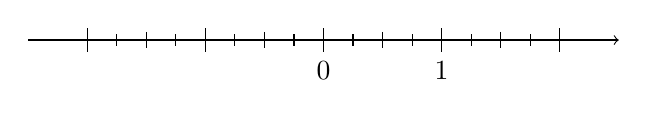
\begin{tikzpicture}[scale=1.5]
\draw[->] (-2.5,0)--(2.5,0);
\foreach \x in {-2,..., 2}{
    \draw (\x,0.1)--(\x,-0.1);
}
\foreach \x in {-2,..., 1}{
    \draw (\x+0.5,0.07)--(\x+0.5,-0.07);
    \foreach \minx in {0.25, 0.5, 0.75}{
        \draw (\x+\minx, 0.05)--(\x+\minx, -0.05);
    }
}
\node[below] at (0,-0.1) {\(0\)};
\node[below] at (1,-0.1) {\(1\)};
\end{tikzpicture}
}

\begin{document}

% =========================================================
% PAGE 1 : VERSION A
% =========================================================

\interroversion{A}

\textbf{Exercice 1 -- Nombres sur une droite graduée \hfill /3}

Sur l'axe gradué ci-dessous, seuls les nombres \(0\) et \(1\) sont indiqués. Placer les nombres suivants :
\[
-1 \qquad \dfrac{3}{2} \qquad -\dfrac{7}{4}
\]

\vspace{1.5cm}

\axegraduepartielle

\vspace{0.5cm}

\textbf{Exercice 2 -- Solution d'une équation \hfill /4}

On considère les deux équations suivantes, d'inconnue \(x\) :
\[
(E_1)\ :\ 2x+1=7 \qquad\qquad (E_2)\ :\ 3x-2=10
\]

Le nombre \(3\) est-il solution de l'équation \((E_1)\) ? de l'équation \((E_2)\) ? Justifier proprement chaque réponse.

\vspace{4cm}

\textbf{Exercice 3 -- Résolution d'équation \hfill /3}

Résoudre l'équation suivante, en détaillant les étapes.
\[
3x-2=7
\]

\vspace{2cm}

\textbf{Exercice 4 -- Intervalles (bonus) \hfill /1}

On considère l'inéquation \((I)\) : \(-3 < x < 2\).

Parmi les quatre intervalles suivants, entourer celui qui correspond exactement à l'ensemble des solutions de \((I)\) :
\begin{center}
\(\left]-3\ ;\ 2\right]\) \hspace{1.5cm} \(\left[-3\ ;\ 2\right[\) \hspace{1.5cm} \(\left]-3\ ;\ 2\right[\) \hspace{1.5cm} \(\left[-3\ ;\ 2\right]\)
\end{center}

\newpage

% =========================================================
% PAGE 2 : VERSION B
% =========================================================

\interroversion{B}

\textbf{Exercice 1 -- Nombres sur une droite graduée \hfill /3}

Sur l'axe gradué ci-dessous, seuls les nombres \(0\) et \(1\) sont indiqués. Placer les nombres suivants :
\[
2 \qquad -\dfrac{1}{2} \qquad \dfrac{5}{4}
\]

\vspace{1.5cm}

\axegraduepartielle

\vspace{0.5cm}

\textbf{Exercice 2 -- Solution d'une équation \hfill /4}

On considère les deux équations suivantes, d'inconnue \(x\) :
\[
(E_1)\ :\ 3x-5=7 \qquad\qquad (E_2)\ :\ 2x+3=13
\]

Le nombre \(4\) est-il solution de l'équation \((E_1)\) ? de l'équation \((E_2)\) ? Justifier proprement chaque réponse.

\vspace{4cm}

\textbf{Exercice 3 -- Résolution d'équation \hfill /3}

Résoudre l'équation suivante, en détaillant les étapes.
\[
2x+5=2
\]

\vspace{2cm}

\textbf{Exercice 4 -- Intervalles (bonus) \hfill /1}

On considère l'inéquation \((I)\) : \(-1 < x < 4\).

Parmi les quatre intervalles suivants, entourer celui qui correspond exactement à l'ensemble des solutions de \((I)\) :
\begin{center}
\(\left[-1\ ;\ 4\right[\) \hspace{1.5cm} \(\left[-1\ ;\ 4\right]\) \hspace{1.5cm} \(\left]-1\ ;\ 4\right]\) \hspace{1.5cm} \(\left]-1\ ;\ 4\right[\)
\end{center}

\newpage

% =========================================================
% PAGE 3 : VERSION C
% =========================================================

\interroversion{C}

\textbf{Exercice 1 -- Nombres sur une droite graduée \hfill /3}

Sur l'axe gradué ci-dessous, seuls les nombres \(0\) et \(1\) sont indiqués. Placer les nombres suivants :
\[
-2 \qquad \dfrac{3}{2} \qquad -\dfrac{3}{4}
\]

\vspace{1.5cm}

\axegraduepartielle

\vspace{0.5cm}

\textbf{Exercice 2 -- Solution d'une équation \hfill /4}

On considère les deux équations suivantes, d'inconnue \(x\) :
\[
(E_1)\ :\ 5x-3=7 \qquad\qquad (E_2)\ :\ 4x+1=17
\]

Le nombre \(2\) est-il solution de l'équation \((E_1)\) ? de l'équation \((E_2)\) ? Justifier proprement chaque réponse.

\vspace{4cm}

\textbf{Exercice 3 -- Résolution d'équation \hfill /3}

Résoudre l'équation suivante, en détaillant les étapes.
\[
-4x+1=9
\]

\vspace{2cm}

\textbf{Exercice 4 -- Intervalles (bonus) \hfill /1}

On considère l'inéquation \((I)\) : \(-4 < x < 0\).

Parmi les quatre intervalles suivants, entourer celui qui correspond exactement à l'ensemble des solutions de \((I)\) :
\begin{center}
\(\left]-4\ ;\ 0\right[\) \hspace{1.5cm} \(\left]-4\ ;\ 0\right]\) \hspace{1.5cm} \(\left[-4\ ;\ 0\right]\) \hspace{1.5cm} \(\left[-4\ ;\ 0\right[\)
\end{center}

\newpage

% =========================================================
% PAGE 4 : VERSION D
% =========================================================

\interroversion{D}

\textbf{Exercice 1 -- Nombres sur une droite graduée \hfill /3}

Sur l'axe gradué ci-dessous, seuls les nombres \(0\) et \(1\) sont indiqués. Placer les nombres suivants :
\[
2 \qquad -\dfrac{3}{2} \qquad \dfrac{7}{4}
\]

\vspace{1.5cm}

\axegraduepartielle

\vspace{0.5cm}

\textbf{Exercice 2 -- Solution d'une équation \hfill /4}

On considère les deux équations suivantes, d'inconnue \(x\) :
\[
(E_1)\ :\ 2x-3=7 \qquad\qquad (E_2)\ :\ 3x+2=20
\]

Le nombre \(5\) est-il solution de l'équation \((E_1)\) ? de l'équation \((E_2)\) ? Justifier proprement chaque réponse.

\vspace{4cm}

\textbf{Exercice 3 -- Résolution d'équation \hfill /3}

Résoudre l'équation suivante, en détaillant les étapes.
\[
5x-3=9
\]

\vspace{2cm}

\textbf{Exercice 4 -- Intervalles (bonus) \hfill /1}

On considère l'inéquation \((I)\) : \(-2 < x < 3\).

Parmi les quatre intervalles suivants, entourer celui qui correspond exactement à l'ensemble des solutions de \((I)\) :
\begin{center}
\(\left[-2\ ;\ 3\right]\) \hspace{1.5cm} \(\left]-2\ ;\ 3\right[\) \hspace{1.5cm} \(\left[-2\ ;\ 3\right[\) \hspace{1.5cm} \(\left]-2\ ;\ 3\right]\)
\end{center}

\end{document}
